

\noindent 
\textbf{\stepcounter{zadatak}
\thecjelina.\thezadatak.}
Blok $m_A = 7\ kg$ položen je na ravni dio klina, a blok $m_B = 15\ kg$ polo\v{z}en je na kosi dio
klina nagiba $\alpha = 37^\circ$.
\begin{enumerate}[label=\alph*)]
 \item Izra\v{c}unajte iznos akceleracije sustava ako pretpostavimo da nema trenja.
 \item Izra\v{c}unajte iznos akceleracije sustava kada je koeficijent kineti\v{c}kog trenja između
blokova i podloge \(\mu_k = 0,1\).
\end{enumerate}
\begin{figure}[h]%{r}{0.35\textwidth} % Inline image example
  \begin{center}
    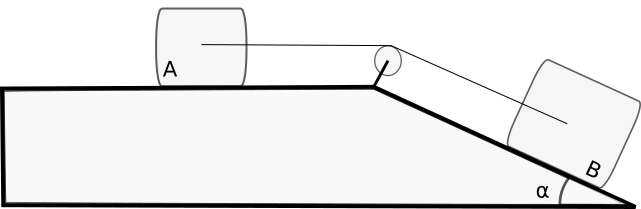
\includegraphics[width=0.5\textwidth]{Dinamika_materijalne_tocke/stol_i_kosina.png}
  \end{center}
  %\caption{Fish}
\end{figure}

